% !TEX root = template.tex

\section{Results}
\subsection{Self-supervised approach: results}

The two-head model was evaluated on the within-domain test split (sets S1--S5,
S7; windows disjoint in time from training) and on the held-out set S6, never
seen during pre-training nor fine-tuning. On the within-domain split the
Activity Recognition head reaches a perfect score, with $100\%$ accuracy and
unitary F1 on all five classes, while the Person Identification head attains
$95.7\%$ accuracy ($\text{F1}=0.958$): the confusion matrix shows that the
residual error is almost entirely a one-directional confusion between P1 and
P2, whereas P3 is never misclassified.

On the held-out set the Activity Recognition head still classifies every
window correctly ($100\%$ accuracy), confirming that the multi-view contrastive
pre-training extracts activity-specific Doppler features that transfer to an
unseen monitor position and acquisition day. The Person Identification head
labels $99.1\%$ of the held-out windows with the correct subject; this figure,
however, must be read as a consistency check rather than a generalization
score, since S6 contains a single subject and therefore does not probe the
discriminative ability of the head. Overall, the two objectives coexist
without interference: the shared representation supports exact activity
recognition while remaining informative enough about the subject, which
indicates that the identity-related component of the signal is not suppressed
by the augmentation pipeline.\\\\
\subsection{Supervised contrastive approach: results}
We now analize the results of the second approach, first on the intra domain test set (S1) and then in order to test the generalization capabilities on six unseen cross-domain scenarios (S2-S7). 
\subsubsection{Intra-domain Performance}
At the individual antenna level, the fine-tuned model achieve an accuracy of 98.8\%, however by applying the Decision Fusion strategy we reach a perfect classification with an accuracy of 99.9\%. This demonstrates that while individual antennas may occasionally misclassify due to noisy signal, the aggregate decision across the four antennas provides an optimal prediction. In figure~\ref{fig:conf1} the confusion matrices of this part.
\begin{figure}[h]
    \centering
    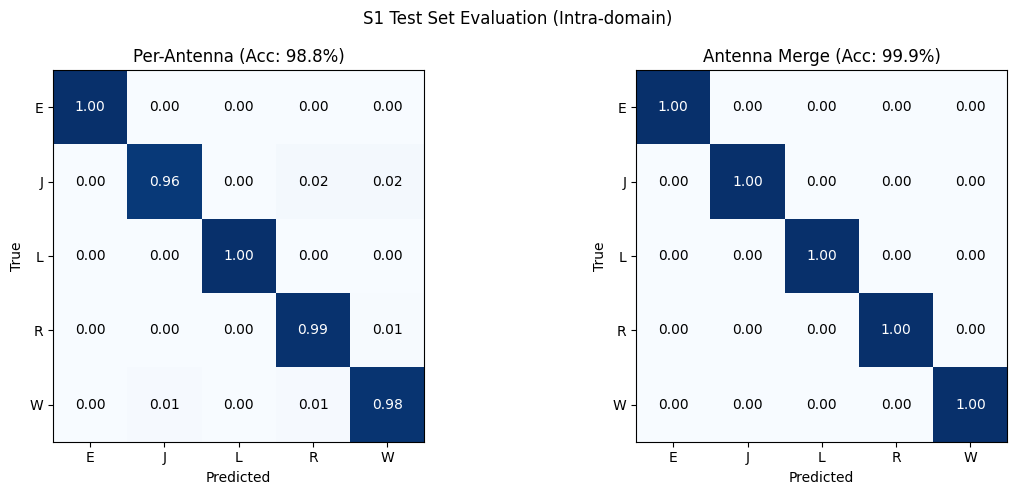
\includegraphics[width=0.4\textwidth]{images/conf1.png}
    \caption{Confusion matrices on the Intra-domain test set S1}
    \label{fig:conf1}
\end{figure}
\subsubsection{Cross-domain Generalization}
In this phase we tested to model on data from environment and subjects never seen during training:
\begin{itemize}
    \item \textbf{Time and subject generalization:} On set S2 (different day, same room) the model maintained an accuracy of 99.89\% while on S3 (both day and subject changed) the accuracy remained at 99.19\%, proving that the contrastive pre-training phase successfully extracted person-independent features.
    \item \textbf{Line of Sight blocked:} In scenarios where the line of Sight was blocked (S4 and S5) the performance stayed above 99\%, indicating the network is capable of identifying activity specific component even when the signal path is attenuated.
    \item \textbf{Environmental Change:} The model showed high robustness to a new room (S6) with 98.36\% accuracy. In the most challenging scenario, S7 (different environment, day, person) resulted in a drop to 89.07\%. The confusion matrix for S7 in figure~\ref{fig:conf2} reveal that the jumping activity is frequently confused with walking, suggesting that significant changes in room geometry and subject simultaneously can shift the Doppler distribution significantly.
\end{itemize}
\begin{figure}[h]
    \centering
    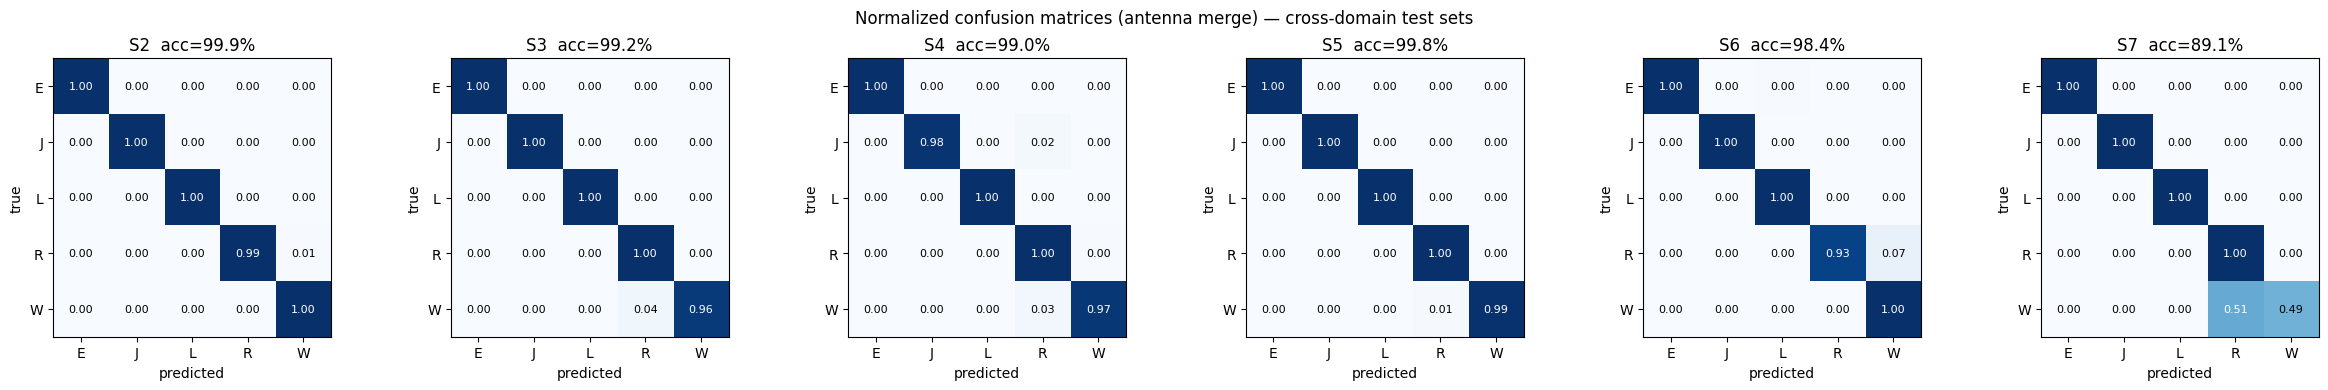
\includegraphics[width=0.5\textwidth]{images/conf2.png}
    \caption{Confusion matrices on the Cross-domain test set}
    \label{fig:conf2}
\end{figure}
In conclusion the mean merged accuracy across all domain test sets was 97.56\%, validating the choice of Supervised Contrastive Learning as a feature extractor that can effectively clusters activity while remaining robust to domain-specific noise.
\label{sec:results}